\subsection{fünftes - bsp e}
Für $ P_e=t^4(t+1)\partial_t^4 + t\partial_t^2+\frac{1}{t}\partial_t+1 $ sieht
das Newton-Polygon wie folgt aus:

\begin{center}
  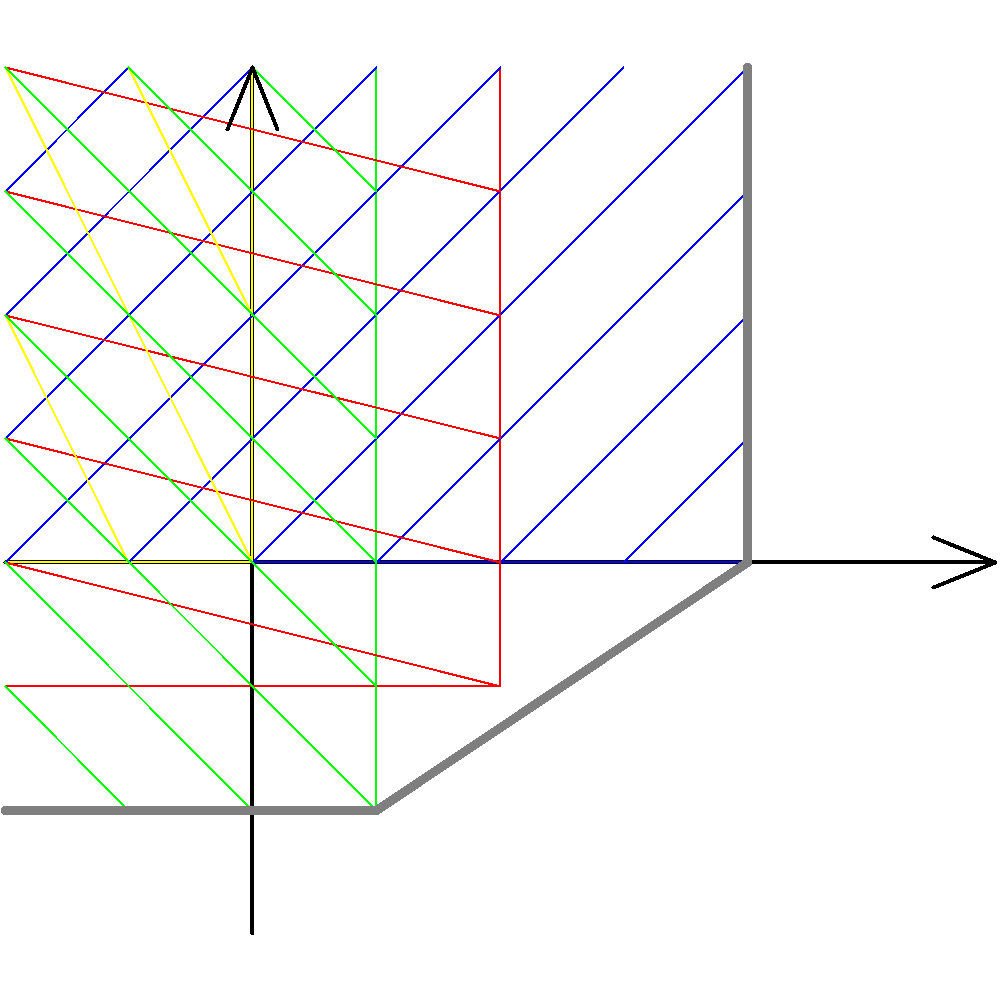
\includegraphics[width=6cm]{img/e.png}
\end{center}

also sind die Slopes $\slopes(P_e)=\{0,\frac{2}{3}\}$.

Dies gilt Analog für das \emph{einfachere}:
\[ \bar P_e=t^4\partial_t^4 +\frac{1}{t}\partial_t \]

\begin{center}
  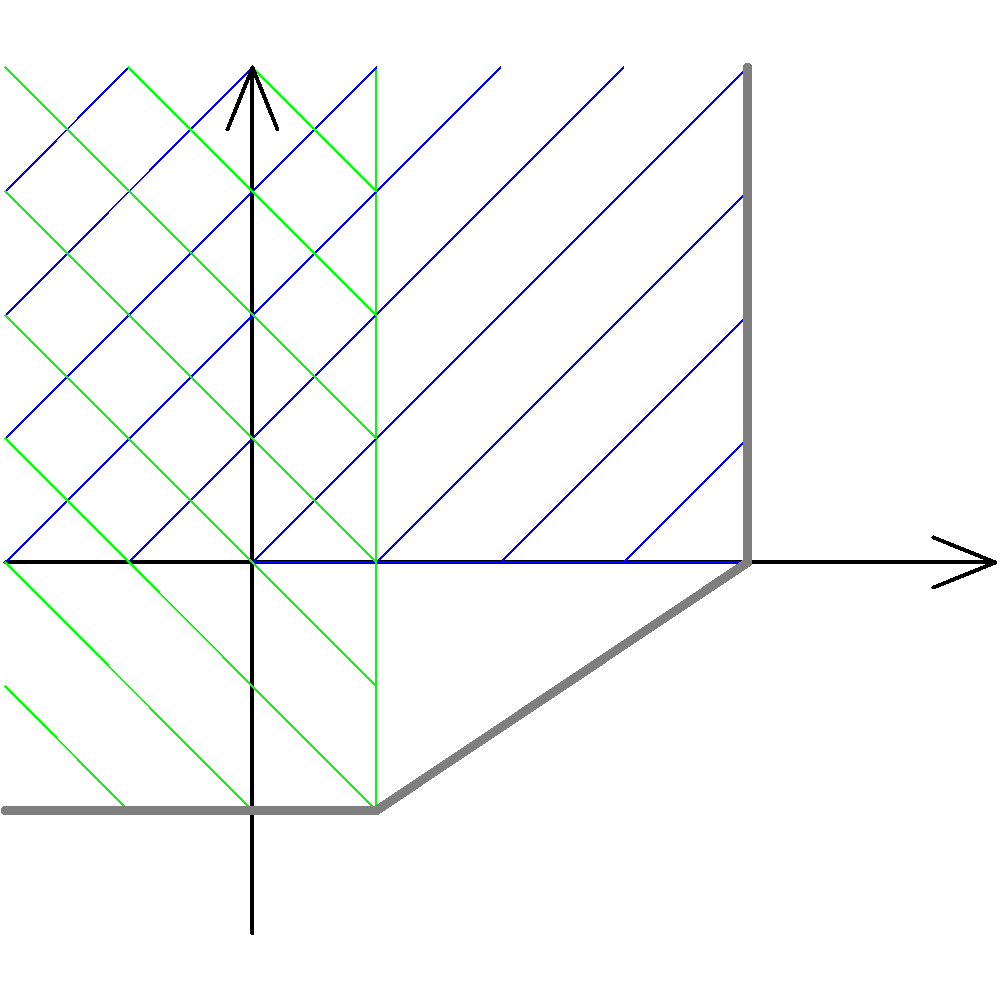
\includegraphics[width=6cm]{img/bar_e.png}
\end{center}
Also offensichtlich gilt $\slopes(\bar P_e)=\{0,\frac{2}{3}\}$, also haben die
Slopes den Hauptnenner $3$, deshalb mache einen Pullback mit $\rho:t\mapsto u^3$

\begin{comment}
  Versuch:
  \[ \rho^+ \bar P_e=u^{12}\partial_u^4 +\frac{1}{u^3}\partial_u \]
  \begin{center}
    FALSCH: $\partial_t\not\mapsto\partial_u$ 
  \end{center}

  $ \rho^+ \bar P_e \Rightarrow
  \begin{cases}
    k=4, l=12 & \Rightarrow u \leq 4, v \geq 8\\
    k=1, l=-3 & \Rightarrow u \leq 1, v \geq -4\\
  \end{cases} $

  \begin{center}
    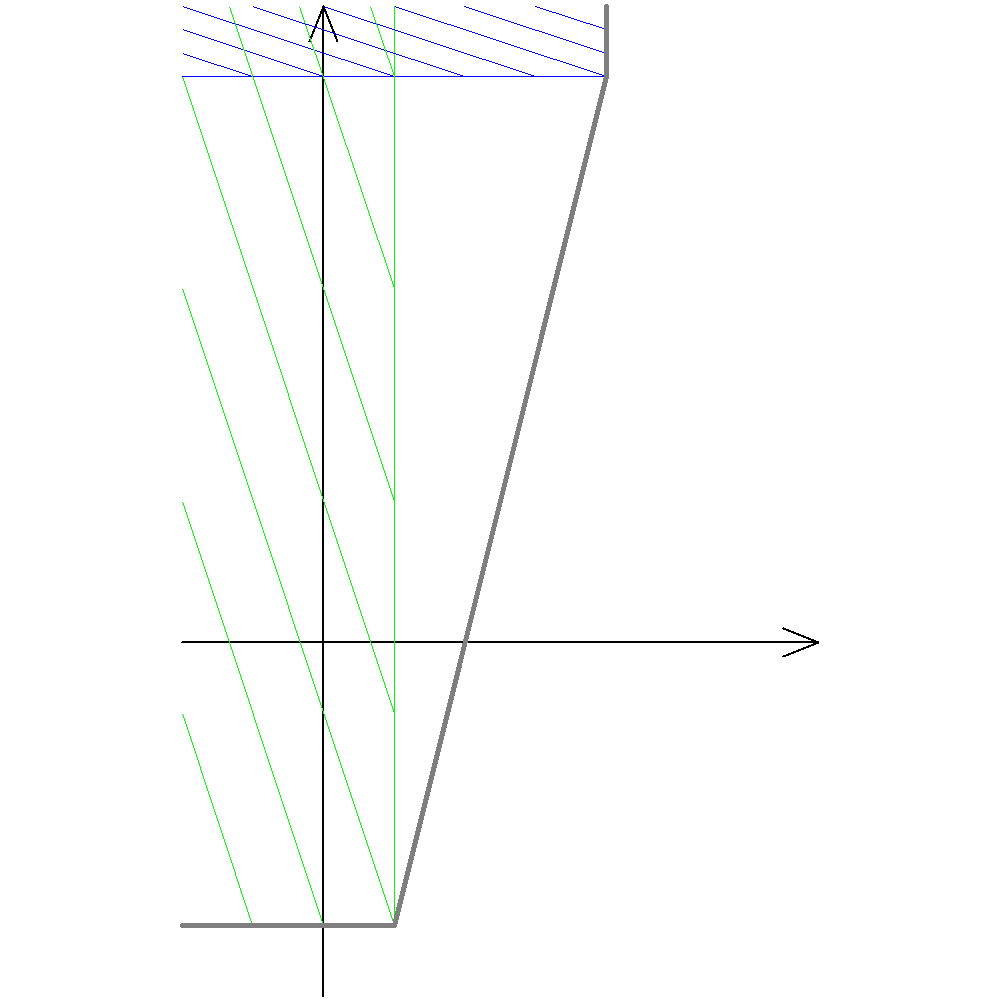
\includegraphics[width=6cm]{img/rho_e.png}
  \end{center}

  \begin{center}
    zu steil
  \end{center}
\end{comment}

% vim: set ft=tex :
